\chapter{\label{ch:2-zvp}The Zero Vector Potential Absorption Mechanism}

\minitoc

\section{Introduction}
Of primary interest in this thesis is the interaction of a relativistically intense short pulse laser interacting with a solid density plasma target with a sharp density gradient. Now is presented the Zero Vector Potential mechanism of attosecond absorption of laser pulse energy, proposed by \textit{Baeva et al} \cite{baeva_2006_TheoryHighorderHarmonic} and later developed by \textit{Savin et al} \cite{savin2017AttosecondscaleAbsorptionExtreme,savin2019EnergyAbsorptionLaserQED}. Laser energy absorption in dense plasmas was first proposed by Wilks and Kruer \cite{wilks1997}, a ponderomotive mechanism where plasma electrons are heated directly by the laser pulse via the so-called $\mathbf{J}\times \mathbf{B}$ force.

%At some point I should briefly chat about other absorption models (I think at the end of the intro - this will also include the stuff above. - Then I will start this chapter by talking about the case where JxB does not apply. ALso in the intro specify that for an overdense plasma, the laser does not propagate and must be reflected and hence we are generally talking about a laser-plasma surface interaction and the implications thereof.) Before this point I also want to discuss preplasmas.

This thesis focuses on the so-called `post-ponderomotive' regime where the frequency of the plasma oscillations ($\omega_p \sim \sqrt{n_e}$) are greater than the $\mathbf{J}\times \mathbf{B}$ induced plasma electron oscillations at $2\omega_L$. The plasma electrons are then fast enough to compensate the ponderomotive pressure of the laser pulse with the formation of electrostatic fields between electrons and ions and so respond adiabatically to the $\mathbf{J}\times \mathbf{B}$ force. Hence plasma electrons cannot be heated directly by the laser pulse. Note that this requires a sufficiently steep density gradient around the relativistic critical density surface (where $S=1$) to shift the main interaction to a region where this condition on the overdensity is satisfied. In this case the ponderomotive pressure of the laser compresses the electrons at the front surface of the plasma and so shifts the laser-plasma surface interaction to plasma densities well beyond the relativistic critical density, leaving behind a positive space charge. This electron-ion charge separation leads to the formation of a \textit{pseudo-capacitor} electrostatic field.


Interestingly working through the condition between $\omega_p$ and $\omega_L$ in normalised units suggests the criterion for this regime is $S > 4$, slightly more constraining than $S>1$ as is typically stated \cite{savin2019thesis}.

% at some point I must be explicitely clear about why this conditoin ad my sims with S=1 are compatible. This above criterion on S is associated with the bunch electrons. For S=1 we observe great compression of the target surface enabling us to enter the regime where the bunch S>4 whilst the bulk remains at S=1. Can thsi also be used to explain the energy absorption in phase one (bunch formation) ? Eneryg can be absorbed by JxB until the bunch density goes above some value???



[Come back to this and write up stuff about actaully it being the relativistc frequncy and critical density surfaces that matter and how this does indeed put a stricter condition on the bulk S value]

So we have entered a regime of adiabaticity where the plasma skin layer is confined within a potential well consisting of the ponderomotive pressure and the Coulomb potential. Consider a relativistic linearly polarised laser pulse obliquely incident, with an angle of incidence of $\theta$, on a semi-infinite plasma, existing for $x>0$. The Hamiltonian of a single electron confined within the potential well \cite{herbert_classical_mechanics} is
\begin{equation}\label{eq:hamiltonian_general}
	\mathcal{H} = c\sqrt{m^2_ec^2 + |\mathbf{p}|^2} - e\Phi.
\end{equation}
Here the first term is the electron energy, $U$, extracted from the invariant of the relativistic 4-momentum of the electron, $\mathbf{P^\mu} = (U/c, \mathbf{p})$,
\begin{equation}
	\mathbf{P^\mu \cdot P_\mu} = \frac{U^2}{c^2} - |\mathbf{p}|^2 = m^2c^2.
\end{equation}
Note that while there has been growing interest in the curvature of spacetime by relativistic lasers [cite edward here], for modern high power lasers this effect is small and not relevant for this thesis. Throughout the inner product of 4-vectors is defined with the Minkowski Metric. [find alex citation on pg 89 of thesis]

The second term of equation \ref{eq:hamiltonian_general} describes the contribution to the electron's energy from the electrostatic potential of the pseudo-capacitor. Decomposing the electron's 3-momentum into orthogonal components: $p_\mathrm{prop}$, along the laser propagation direction, $p_\mathrm{pol}$, along the polarisation axis of the laser pulse and $p_\perp$, perpendicular to both, two simplifications can be made. Firstly, by canonical conservation of transverse momentum, $p_\mathrm{pol} = eA$, where $A$ is the laser vector potential. Secondly, in the case of a $p$-polarised laser pulse (the known optimum for ZVP electron bunch generation), the forces at play confine the electron trajectory to the  $p_\mathrm{prop}$-$p_\mathrm{pol}$ plane and the interaction geometry is in essence \ac{2D}.

[include a diagram alluding to this?-it is basically since B is out of the plane and all other E fields are in the plane, also perhaps provide a foot not here to explain how incidentally this all provides a succinct explanation of why p is better?]

Explicitly, the Hamiltonian is now
\begin{equation}\label{eq:hamiltonian_specific}
	\mathcal{H} = c\sqrt{m^2_ec^2 + p^2_\mathrm{prop} + e^2A^2} - e\Phi.
\end{equation}
From equation \ref{eq:hamiltonian_specific} it is clear that should the vector potential pass through zero, one of the walls of the potential well is suppressed, allowing electrons in the in the skin layer to escape the plasma, breaking adiabaticity. The necessity of vector potential zeros for this violent reconstruction of the plasma surface led Baeva et al \cite{baeva2011ZeroVectorPotential} to coin the term `Zero Vector Potential' mechanism to describe this process. Indeed, while in standard calculations a laser pulse will exponentially decay within a skin layer without passing through zero, Baeva et al \cite{baeva2011ZeroVectorPotential} were able to demonstrate in \ac{PIC} simulations that for this regime, zeros are able to propagate through the skin layer of the plasma. The explanation for this difference in mechanics relies on a Doppler shift in the laser field due to the relativistic motion of the ablating plasma surface, and the mathematical formalism of this process proceeds as follows.

[I think before this point it would be good to enter in the language of electron bunches or sheaths - I will continue the dicussion assuming this concept has been introduced].

As the \ac{ZVP} mechanism is a relativistic phenomenon, it is essential to consider the laser pulse propagating through a relativistically ablating electron bunch (i.e. with some component of its velocity anti-parallel to the laser pulse propagation direction). Transforming to the rest frame of the ablating front, beyond the relativistic critical density surface, the vector potential of the laser pulse will be an evanescent wave, at the spatial centre of the laser pulse, it can be described simply by
\begin{equation}
	\mathbf{A}'_\mathrm{L}(t',r') = A'_0\cos(\omega'_\mathrm{L}t')\exp(-r'/\delta')\hat{\mathbf{r}}'_\mathrm{pol}= A'_\mathrm{L}\hat{\mathbf{r}}'_\mathrm{pol},
\end{equation}
where the primed symbols indicate that these quantities are measured in the rest frame of the expanding front, $A'_0$ is the vector potential amplitude and $\omega'_\mathrm{L}$ is the frequency of the laser pulse, $r'$ is the propagation distance of the laser into the plasma, $\delta'$ is the skin depth and $\hat{\mathbf{r}}'_\mathrm{pol}$ a unit vector defining the polarisation direction of the laser pulse. Un-primed coordinates will indicate the lab frame measurements.

[For sure include a diagram of this]

While in previous demonstrations of the vector potential zeros, it was assumed that the ablation occurs normal to plasma surface, it is now known that this ablation occurs in the specular reflection direction and it is necessary to confirm that zeros are still predicted. Consider a p-polarised laser pulse confined to the $x$-$y$ plane incident with an angle of incidence $\theta$ on an ablating overdense plasma expanding with velocity $-v_f\hat{\mathbf{x}}$ in the lab frame, as in figure \ref{fig:zvp_ablatingfront}.
% TODO: \usepackage{graphicx} required
\begin{figure}
	\centering
	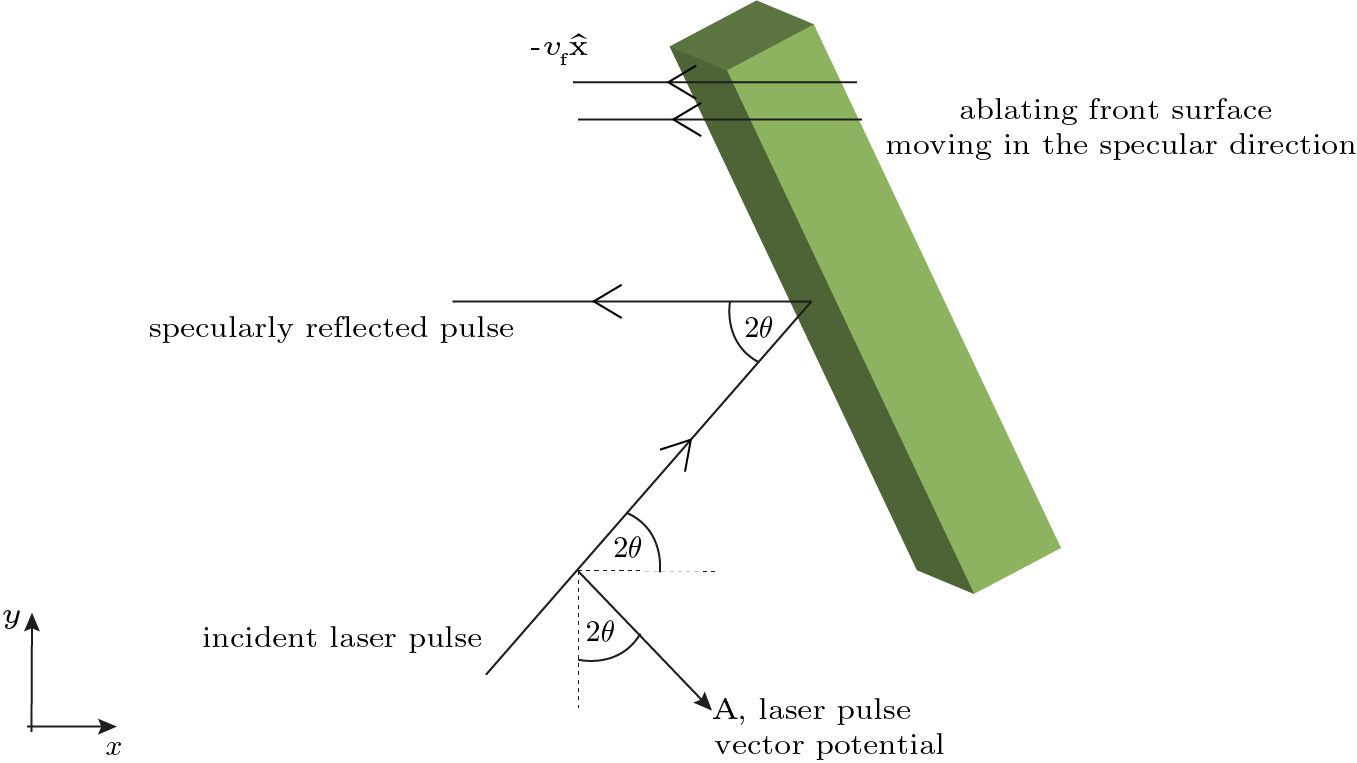
\includegraphics[width=0.7\linewidth]{figures/zvp/zvp_ablating_front}
	\caption{Diagram of a $p$-polarised laser pulse incident on an ablating overdense plasma. The laser is incident obliquely at an angle of $\theta$ and is reflected specularly. The plasma ablates specularly also. The interaction geometry is confined to a 2D plane.}
	\label{fig:zvp_ablatingfront}
\end{figure}
The direction of polarisation is
\begin{equation}
	\hat{\mathbf{r}}_\mathrm{pol} = \hat{\mathbf{x}}\sin{2\theta} - \hat{\mathbf{y}}\cos{2\theta}
\end{equation}
and the velocity of the rest frame of the ablating front relative to the lab frame is $-v_f\hat{\mathbf{x}}$.

Applying the Lorentz transformation to the electromagnetic 4-potential,
\begin{equation}
	\mathbf{A}_\mu = (\phi/c,\mathbf{A}),
\end{equation}
explicitly,
\begin{equation}
	\mathbf{A}'_\mu = \Lambda^\mu_\nu \mathbf{A}_\nu,
\end{equation}
where $\Lambda^\mu_\nu$, the Lorentz transform in this geometry is
\begin{equation}\label{eq:zvp_lorentz}
	\Lambda^\mu_\nu = \begin{pmatrix}
			\gamma & -\beta\gamma & 0 & 0\\
			-\beta\gamma & \gamma & 0 & 0\\
			0 & 0& 1 & 0\\
			0 & 0 & 0 & 1
	\end{pmatrix}
\end{equation}
and here $\beta = -v_\mathrm{f}/c$, $\gamma = 1/\sqrt{1-\beta^2}$. Immediately from the $y$-coordinate transformation,
\begin{equation}\label{eq:zvp_lorentz_y}
	A'_\mathrm{L}\cos{2\theta'} = A_\mathrm{L}\cos{2\theta}.
\end{equation}
Applying the headlight effect for a source moving at an angle $2\theta$ to the boosted frame,
\begin{equation}
	\cos{(2\theta')} = \frac{\cos{(2\theta)}-\beta}{1 - \beta\cos{(2\theta)}}
\end{equation}
and rearranging equation \ref{eq:zvp_lorentz_y}, the vector potential in the lab frame is
\begin{equation}\label{eq:zvp_labA}
	A_\mathrm{L} = \frac{1-\beta \sec{(2\theta)}}{1 - \beta\cos{(2\theta)}} A'_0\cos{(\omega'_L t')}\exp{(-r'/\delta')}.
\end{equation}
Writing the boosted frame space-time coordinates in terms of the lab frame coordinates,
\begin{equation}
	ct' = \gamma(ct-\beta x),
\end{equation}
\begin{equation}
	x' = \gamma(x-\beta ct),
\end{equation}
yields
\begin{equation}\label{eq:zvp_labAfull}
	A_\mathrm{L} =  A_0\cos{(\omega_L t - kx)}\exp{\left(-\frac{\sqrt{(x-\beta ct)^2+(y/\gamma)^2}}{\delta}\right)},
\end{equation}
where
\begin{equation}
	A_0 = \frac{1-\beta \sec{(2\theta)}}{1 - \beta\cos{(2\theta)}}A'_0,
\end{equation}
\begin{equation}
	\omega_L = \gamma \omega'_L,
\end{equation}
\begin{equation}
	k = \frac{\beta \gamma\omega'_L}{c},
\end{equation}
\begin{equation}
	\delta = \frac{\delta'}{\gamma}.
\end{equation}
The oscillatory term in equation \ref{eq:zvp_labAfull} demonstrates the propagation of vector potential zeros within the plasma target. From the structure of this term it would appear that these zeros are expelled from the plasma along the specular direction at a speed (recall beta is negative - change this earlier in the theory so that that negative sign is more explicit in the result.)
\begin{equation}
	v_\phi = \frac{\omega_L}{k} = \frac{c}{\beta} = -\frac{c^2}{v_\mathrm{f}}.
\end{equation}
Could also discuss here about how relativistic similarity theory derives that zeros move at speed c but how that cannot be valid since then we would always have infinitely thin radiation pulses, unless there is an extended range of zero? I suppose there is some radiation happening around the peak? Good questions..
One remaining consideration is we require that the zero gets through the whole electron bunch which is generally at very high density but is also very thin, in a way is this skin depth not what precisely determines the bunch width? The bunch will be compressed until the skin depth goes to zero across it perhaps? Things to think about.


Qualitatively, and in summary, for sufficiently intense laser pulses, electrons on the radiated surface of a solid target are accelerated by the laser to relativistic velocities at a fraction of a laser pulse cycle and therefore electrons both follow similar trajectories and are able to respond adiabatically to the $\mathbf{J}\times \mathbf{B}$ force of the laser pulse. They therefore form a high charge density thin coherent electron sheath on the front surface of the plasma but displaced inwards from the immobile ions (ions are approximately immobile on the timescale of a laser pulse cycle) via the ponderomotive pressure of the laser. This charge separation generates a longitudinal electrostatic pseudocapacitor field that confines electrons to a potential well on the front surface of the plasma, preventing further propagation of the electron bunch into the plasma bulk. When the zero of the vector potential passes through the electron bunch, the ponderomotive pressure instantaneously vanishes and electrons are ejected specularly from the target, copropagating with the zeroes and gaining energy as they discharge the pseudocapacitor field. Coherent sychrotron emission occurs concurrently. The electron bunch is then rotated by the laser pulse and launched into the bulk at high energy.


SOmething to think about: which comes first? electron bunch acceleration across pseudo capacitor or zeros?
Laser accelerates electorns in laser propagation direction , however cannot propagate further into the plasma so only get motion parallel to surface, once potentail well disrupted, accleration is perp to surface so combined, electrons travel in specular direction.
So actually what we are saying is the zeros will go in whatever direction the surface ablates in, but the surface will move in a direction dependent on the components of electron 


\subsubsection{The headlight effect}\label{sec:zvp_headlight}
This most likely goes in the appendix. But storing here for now.

The headlight effect describes the beaming of an isotropically emitting source travelling at some velocity relative to an observer. Consider the geometry of figure \ref{fig:zvp_ablatingfront} with the source (the laser pulse) travelling at an angle $2\theta$ to the observer (in this case, the ablating front). A photon with energy $E$ emitted from the rest frame of the source (in this case the lab frame) has a 4-momentum
\begin{equation}
	\mathbf{P}_\mu = \left(\frac{E}{c},\frac{E}{c}\cos{2\theta},\frac{E}{c}\sin{2\theta}\right).
\end{equation}
As the interaction geometry is confined to a 2D plane,  the $z$-component can be safely neglected. Applying the lorentz boost of equation \ref{eq:zvp_lorentz},
\begin{equation}
	\begin{split}
		\frac{E'}{c} = \gamma \left( \frac{E}{c} - \beta \frac{E}{c}\cos{2\theta}\right) \\
		\frac{E'}{c}\cos{2\theta'} = \gamma \left( \frac{E}{c}\cos{2\theta} - \beta \frac{E}{c}\right).
	\end{split}
\end{equation}
Solving these equations for the angle in the boosted frame,
\begin{equation}
	\cos{2\theta'} = \frac{\cos{2\theta} - \beta}{1-\beta\cos{2\theta}}.
\end{equation}

\subsubsection{Conservation of generalised transverse momentum}\label{sec_app_conservation-generalised-mometum}
This should most likely go in the appendix/ before ZVP Hamiltonian discussion.

Whilst it is commonly stated within the field of laser-solid interactions, it would appear that some nuance/detail is missing from the discussion which in turn shrouds the \ac{ZVP} mechanism in confusion.

Consider a holonomic system of N relativistic particles under the influence of electromagnetic forces. A particle $j$ with charge $e_j$ and mass $m_\mathrm{j}$ experiences a scalar potential,
\begin{equation}
	U_{j} = e_j(\Phi - \mathbf{A} \cdot \mathbf{v}_{j})
\end{equation}
and hence the system is described by the Lagrangian
\begin{equation}
	L = \sum^N_{j=1}\left( - m_\mathrm{j}c^2\sqrt{1-\beta^2_\mathrm{j}} - e_j(\Phi - \mathbf{A} \cdot \mathbf{v}_\mathrm{j}) \right),
\end{equation}
where $\beta^2 = \mathbf{v}_\mathrm{j}\cdot\mathbf{v}_\mathrm{j} /c^2$ \cite{goldstein_classical_mechanics}.
The generalised momentum corresponding to coordinate $x_j$ is
\begin{equation}
	p_{j,x} = \frac{\partial L}{\partial \dot{x}_j} = m_j\dot{x}_j + e_jA_x,
\end{equation}
explicitely, the generalised momentum describes both the linear mechanical momentum and the momentum of the electromagnetic field. Via Noether's theorem, if $L$ is independent of $x_j$, \textit{i.e.} spatially homogeneous along $x$ for particle $j$, then 
\begin{equation}
	\dot{p}_{j,x} = 0.
\end{equation}
Considering a p-polarised Gaussian laser pulse, axis of polarisation along $x$, $A_x$ will be approximately constant. Integrating and noting that initially there is no linear or electromagnetic momentum, the generalised transverse momentum conservation equation for an electron at the plasma-vacuum boundary is obtained, namely,
\begin{equation}
	p_\mathrm{T} = eA,
\end{equation}
where $p_mathrm{T}$ is the electron momentum along the polarisation axis of the laser pulse. and $A$ its vector potential.

Note that this is only valid provided the radiating electron does not radiate along the direction of $\mathbf{A}$ as discussed by Sokolov \textit{et al} \cite{sokolov_2009_DynamicsEmittingElectrons}. But we do know this radiation is specular so this is true for normal incidence but not specular?? Really need to consider what the EM fields are in the surface from combined Incident and reflected.
The implications of this should maybe be considered?? Also note that this is only true for gaussian pulses with spatial profiles $\gg$ than electron trajectories (\textit{i.e.} twice the relativistic larmor radius).

\subsection{ZVP electron bunch energies}\label{sec:zvp_energies_derivation}
In \cite{baeva_2011_ZeroVectorPotential}, Baeva \textit{et al} propose energy scalings for electron bunches produced in the \ac{ZVP} regime as a function of the laser intensity and plasma density, finding that one of the key statements of similarity theory ($p \sim a_0 S^x$, where $x$ is some integer value, THIS NEEDS A CITE I THINK IT APPEARS IN BAEVAS ORIGINAL HHG PAPER) holds for the \ac{ZVP} mechanism. Later this was then extended to \ac{3D} by Savin \textit{et al} \cite{savin_2017_AttosecondscaleAbsorptionExtreme}. What follows is that discussion with a more close consideration of the both consequences and constants of proportionality.

(Pherhaps I should redo this discussion condering infinitessimal areas of the plasma surface to show how variation can exist across the surface) Defo do this! And say that provided the variation is small, rel to what though? the surface remains approximately flat -> that is totally not true

Consider again the semi-infinite block of plasma proposed in figure \ref{fig:zvp_ablatingfront}, normally irradiated by a laser pulse with wavelength $\lambda_\mathrm{L}$ and peak electric field, $E_\mathrm{L}$. It is now the ponderomotive pressure of the laser that displaces the electron fluid. Consider ust one laser cycle. The electron surface moves inwards until the pressure exerted by the peak instantaneous ponderomotive pressure of the laser pulse cycle,
\begin{equation}
	\mathbf{P}_\mathrm{L} = \epsilon_0 E^2_\mathrm{L} \hat{\mathbf{x}} = \epsilon_0 \left(\frac{a_0\omega_\mathrm{L}m_\mathrm{e}c}{e}\right)^2 \hat{\mathbf{x}}
\end{equation}
is equal and opposite to the pressure exerted by the pseudo-capacitor field,
\begin{equation}
	\mathbf{P}_\mathrm{C} = \frac{QE}{\sigma} \hat{\mathbf{x}}= -\frac{(en_\mathrm{e}\Delta x)^2}{\epsilon_0}\hat{\mathbf{x}}
\end{equation} 
using equations \ref{eq:intro_Q} and \ref{eq:intro_E}. Equating the magnitudes of $\mathbf{P}_\mathrm{L}$ and $\mathbf{P}_\mathrm{C}$, the maximum displacement inwards of electrons is
\begin{equation}\label{eq:zvp_dx}
	\Delta x \hat{\mathbf{x}} = \frac{c}{\omega_\mathrm{L}}\frac{a_0}{\bar{n}_\mathrm{e}}\hat{\mathbf{x}}  = \frac{1}{kS}\hat{\mathbf{x}},
\end{equation}
where $k$ is the wave-vector of the laser pulse. Correspondingly,
\begin{equation}\label{eq:zvp_E}
	E = \frac{en_\mathrm{e}}{\epsilon_0}\Delta x = \frac{\omega_\mathrm{L}cm_\mathrm{e}a_0}{e} = E_\mathrm{L}.
\end{equation}
Applying the results of equations \ref{eq:zvp_dx} and \ref{eq:zvp_E}, when the ponderomotive pressure vanishes and the electron bunch is launched across the pseudo-capacitor, the relativistic kinetic energy gained by a single electron is
\begin{equation}\label{eq:zvp_T}
	T =  \int \mathbf{F}\cdot\mathrm{d}\mathbf{s} = \int^0_{\Delta x} -eEdx = \int^0_{\Delta x}-\frac{en_\mathrm{e}x}{\epsilon_0}dx = \frac{1}{2}m_\mathrm{e}c^2\frac{a^2_0}{\bar{n}_\mathrm{e}}
\end{equation}
or an electron gamma factor,
\begin{equation}
	\gamma = \frac{1}{\sqrt{1-\beta^2}} = 1 + \frac{a_0^2}{2\bar{n}_\mathrm{e}}.
\end{equation}
Assuming all displaced electrons are captured by the pseudo-capacitor field and launched as a coherent bunch, the total kinetic energy of the electron bunch is
\begin{equation}\label{eq:zvp_U}
	U_\mathrm{ZVP} = n_\mathrm{e}\sigma\Delta x T = \frac{\sigma n_\mathrm{c}}{k}\times m_\mathrm{e}c^2 \frac{a^3_0}{\bar{n}_\mathrm{e}}.
\end{equation}
It is now interesting to compare equation \ref{eq:zvp_U} to the laser energy deposited upon the plasma surface and therefore consider what fraction of the laser energy can be absorbed via the \ac{ZVP} mechanism. Using $E = E_\mathrm{L}$, \ref{eq:zvp_U} can be rewritten as
\begin{equation}
	U_\mathrm{ZVP} = \frac{1}{2\omega_\mathrm{L} S}\sigma c \epsilon_0 E^2_\mathrm{L}.
\end{equation}
For the case of normal incidence, bunches are produced at a frequency of $2\omega_\mathrm{L}$, naturally following the frequncy of the $\mathbf{J}\times \mathbf{B}$ force. Assuming a sinusoidal plane wave incident with surface area $\sigma$, the energy absorbed in half a laser cycle is
\begin{equation}
	 U_\mathrm{L,1/2} = \sigma \frac{T}{2}\langle I_\mathrm{L}\rangle = \frac{2\pi}{4\omega_\mathrm{L}}\sigma c\epsilon_0E^2_\mathrm{L}.
\end{equation}
Hence,
\begin{equation}
	\eta_\mathrm{ZVP} = \frac{U_\mathrm{ZVP}}{U_\mathrm{L,1/2}} = \frac{1}{\pi S}.
\end{equation}
Interestingly, this new analytical result predicts the trend observed by A. Savin \cite{savin_2019_ModellingLaserPlasmaInteractions} in \ac{PIC} simulations both in magnitude and in scaling. Indeed, A. Savin demonstrated 
\begin{equation}
	\eta_\mathrm{ZVP} \sim S^{-1.000(3)},
\end{equation}
however, this result led A. Savin to conclude increasing $S$ increases the energy in the reflected \ac{HHG} beam thus increasing high harmonic efficiency, seemingly in tension with the vast majority of the work on this regime [CITE CITE CITE]. The resolution arises from the follwoing: there are two distinct conversion efficiencies which describe the reflected harmonic spectrum. The conversion efficiency into the whole reflected beam and the conversion efficiency into individual harmonics. While the total conversion into reflected beam decreases for decreasing $S$, the slope of the harmonic spectrum also decreases and therefore while A. Savin is absolutely correct, the imporant parameter (the slope of the harmonic spectra) follows the opposite trend.

Indeed high X-ray harmonic efficiency neccesitates high inefficiencies in the production of ZVP electron bunches as higher energy bunches produce more coherent reflected radiation, a caveat not often considered in the quest for higher-order harmonics.



Next up: the unification of RES and ZVP.

Also mention alex's piont about using 2D simulations.


Earlier write something along the lines of explaining while ZVP absorption does represent laser energy absorption, bulk heating occurs rather indirectly.


Perhaps derive equivalence between res and ZVP here?


Then section of a typical bunch properties

Then Energy scalings

Then QED?
Then experiment?



